% SPDX-License-Identifier: CC-BY-4.0
% Figure 4 - representative storage-and-retrieval cycle, t = 0 at the herald.
% Reconstructed from Buser et al. 2022 (Section V, Fig. 4) and the HeraldRT
% register defaults. Conceptual: NOT a measurement of HeraldRT.
% Value classes: P published, D derived from the paper, C configurable, A assumption.
\documentclass[tikz, border=0pt]{standalone}
% SPDX-License-Identifier: CC-BY-4.0
% styles.tex - shared typography, colours and TikZ styles for all HeraldRT figures.
%
% Conventions used in every figure
%   optical path        red, solid, 1.2pt, open arrow head
%   electrical event    blue, solid, 0.9pt (detector pulses, herald)
%   control output      green, dashed, 0.9pt (electronics -> actuators)
%   host / config       grey, dotted
%   implemented block   solid outline     proposed block   dashed grey outline
%   asynchronous domain light amber fill  synchronous domain light blue fill

\usepackage{fontspec}
\usepackage{unicode-math}
\setmainfont{FiraSans}[
  Extension = .otf, UprightFont = *-Book, BoldFont = *-SemiBold,
  ItalicFont = *-BookItalic, BoldItalicFont = *-SemiBoldItalic]
\setsansfont{FiraSans}[
  Extension = .otf, UprightFont = *-Book, BoldFont = *-SemiBold,
  ItalicFont = *-BookItalic, BoldItalicFont = *-SemiBoldItalic]
\setmathfont{FiraMath-Regular.otf}
\setmonofont{FiraMono}[Extension = .otf, UprightFont = *-Regular, BoldFont = *-Medium,
  Scale = 0.92]
\renewcommand{\familydefault}{\sfdefault}

\usepackage[detect-all]{siunitx}
\sisetup{range-phrase = --, range-units = single, per-mode = symbol}

\usepackage{tikz}
\usetikzlibrary{arrows.meta, positioning, calc, fit, backgrounds,
  decorations.pathmorphing, decorations.markings, shapes.geometric, shapes.misc}

% layer for domain shading: above the white page, below blocks and wires
\pgfdeclarelayer{board}
\pgfdeclarelayer{domains}
\pgfsetlayers{background, board, domains, main}

% reproducible PDF (no creation date / ID differences between builds)
\pdfvariable suppressoptionalinfo 1023

% ------------------------------------------------------------------ colours
\definecolor{ink}{HTML}{1B2631}
\definecolor{optical}{HTML}{B03A2E}
\definecolor{opticallight}{HTML}{F2D7D5}
\definecolor{pumpviolet}{HTML}{6C3483}
\definecolor{elec}{HTML}{1F4E79}
\definecolor{ctrl}{HTML}{1E7B4A}
\definecolor{host}{HTML}{6E7B85}
\definecolor{asyncfill}{HTML}{FDF2E3}
\definecolor{asyncline}{HTML}{C07A1E}
\definecolor{syncfill}{HTML}{EAF2FA}
\definecolor{syncline}{HTML}{4F7FAF}
\definecolor{boxfill}{HTML}{FFFFFF}
\definecolor{muted}{HTML}{8A949C}
\definecolor{lat}{HTML}{C0392B}

\colorlet{proposed}{muted}

% ------------------------------------------------------------------ styles
\tikzset{
  every picture/.style = {line join = round, line cap = round, font = \small,
    text = ink, >={Stealth[length=2.2mm, width=1.6mm]}},
  % white page so the SVG stays readable in GitHub's dark mode
  white page/.style = {show background rectangle,
    background rectangle/.style = {fill = white, draw = none},
    inner frame xsep = 4mm, inner frame ysep = 3.5mm},
  % blocks
  block/.style = {draw = ink, line width = 0.7pt, fill = boxfill, rounded corners = 1.5pt,
    align = center, inner sep = 4pt, minimum height = 9mm},
  smallblock/.style = {block, font = \footnotesize, minimum height = 7mm, inner sep = 3pt},
  proposedblock/.style = {block, draw = proposed, dash pattern = on 3pt off 2pt,
    text = proposed, fill = white},
  device/.style = {block, fill = black!3},
  domain async/.style = {draw = asyncline, fill = asyncfill, line width = 0.6pt,
    rounded corners = 3pt, inner sep = 3.5mm},
  domain sync/.style = {draw = syncline, fill = syncfill, line width = 0.6pt,
    rounded corners = 3pt, inner sep = 3.5mm},
  board/.style = {draw = ink!70, line width = 0.7pt, rounded corners = 4pt, inner sep = 4mm},
  domain label/.style = {font = \footnotesize\bfseries, align = left},
  note/.style = {font = \footnotesize, text = ink!80, align = center},
  tag/.style = {font = \scriptsize, text = ink!70},
  % signals
  optical/.style = {draw = optical, line width = 1.2pt, -{Stealth[length=2.6mm, width=2mm]}},
  optical nohead/.style = {draw = optical, line width = 1.2pt},
  pump light/.style = {draw = pumpviolet, line width = 1.2pt, -{Stealth[length=2.6mm, width=2mm]}},
  elec/.style = {draw = elec, line width = 0.9pt, ->},
  ctrl/.style = {draw = ctrl, line width = 0.9pt, dash pattern = on 3.5pt off 2pt, ->},
  hostlink/.style = {draw = host, line width = 0.8pt, dash pattern = on 1pt off 1.6pt, <->},
  latency/.style = {circle, fill = lat, text = white, font = \scriptsize\bfseries,
    inner sep = 0.6pt, minimum size = 3.9mm},
}

% value-class tags used in the timing figure
\newcommand{\clsP}{\textsuperscript{\textcolor{optical}{\bfseries P}}}
\newcommand{\clsD}{\textsuperscript{\textcolor{asyncline}{\bfseries D}}}
\newcommand{\clsC}{\textsuperscript{\textcolor{ctrl}{\bfseries C}}}
\newcommand{\clsA}{\textsuperscript{\textcolor{host}{\bfseries A}}}


\begin{document}
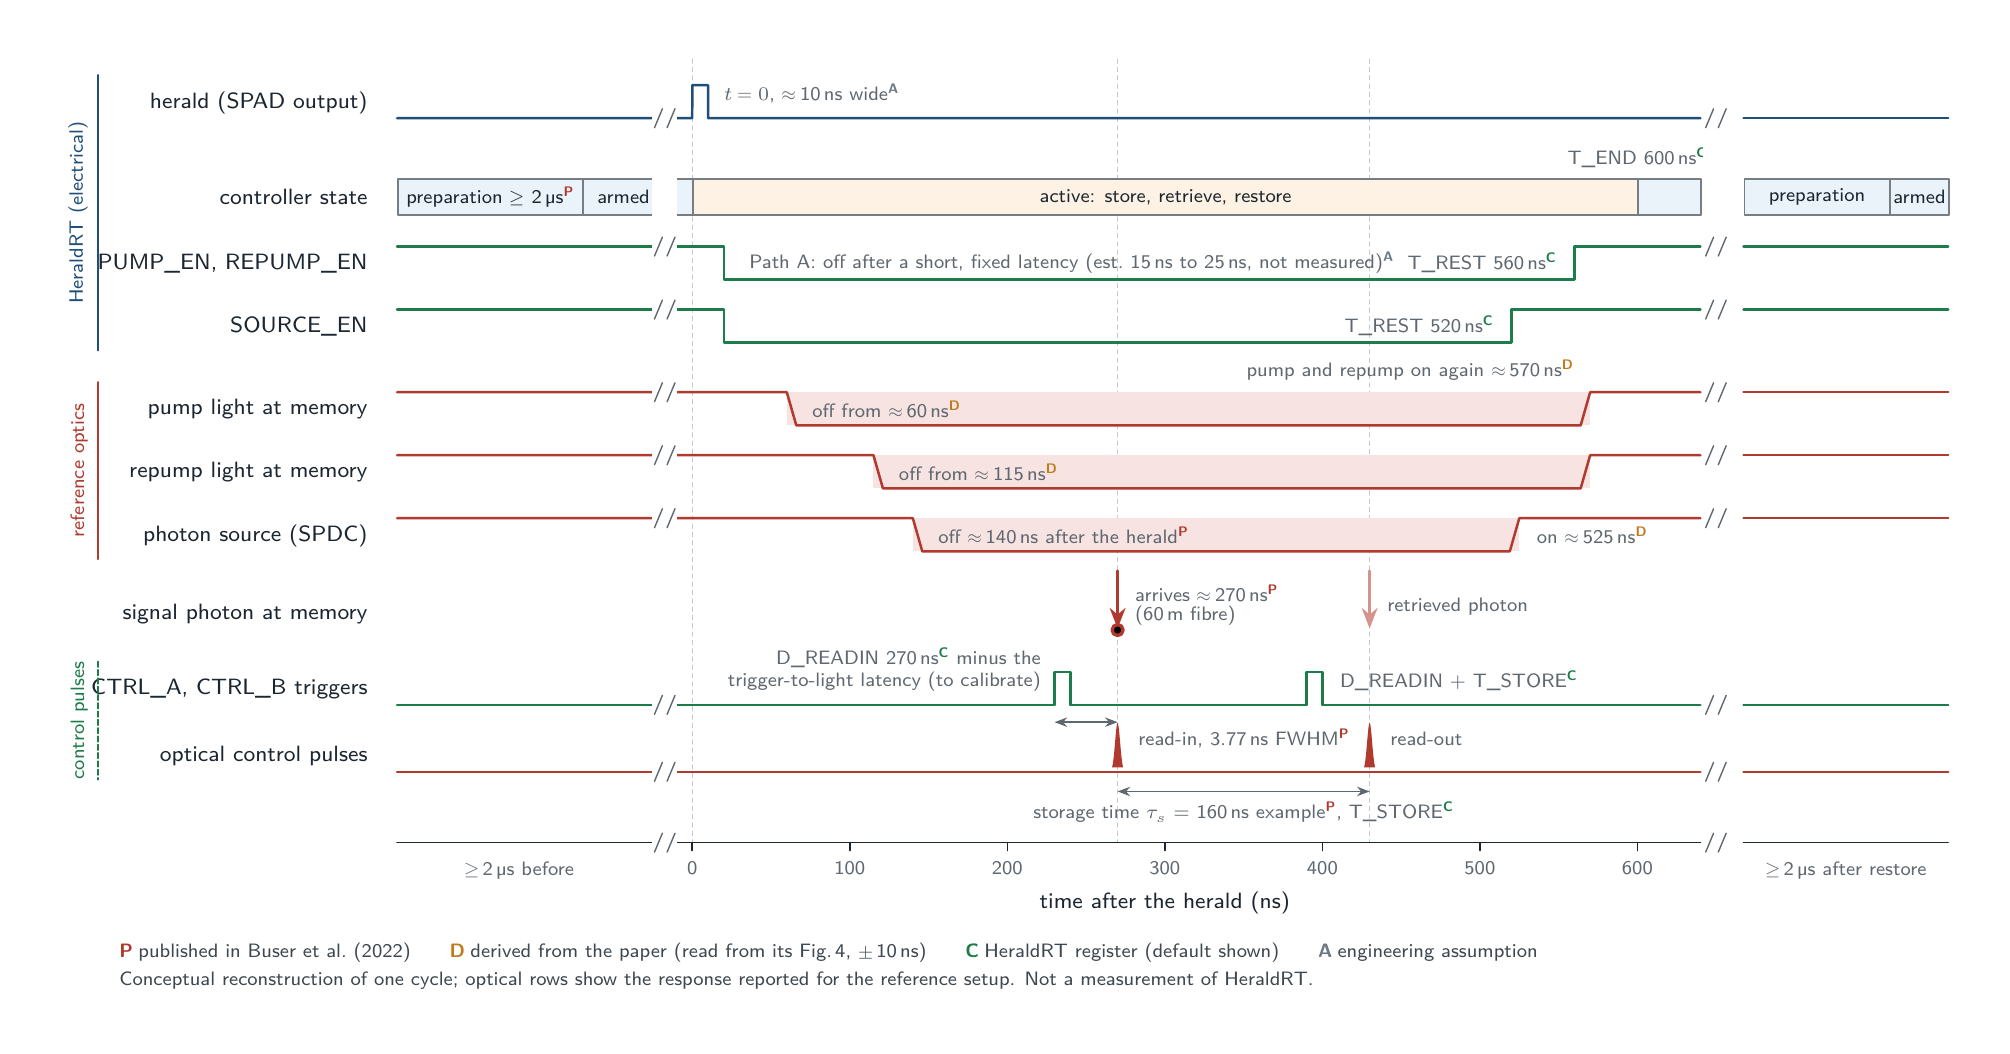
\begin{tikzpicture}[white page, x = 1cm, y = 1cm]
  \def\s{0.02}          % cm per ns in the main window
  \def\h{0.42}          % waveform height
  \pgfmathsetmacro{\xmin}{-60*\s}
  \pgfmathsetmacro{\xmax}{640*\s}
  \tikzset{
    rowlabel/.style = {anchor = east, font = \footnotesize, align = right},
    wave/.style  = {line width = 0.9pt},
    ewave/.style = {wave, draw = elec},
    cwave/.style = {wave, draw = ctrl},
    owave/.style = {wave, draw = optical},
    offband/.style = {fill = opticallight!70, draw = none},
    dim/.style = {draw = ink!70, line width = 0.5pt, {Stealth[length=1.6mm]}-{Stealth[length=1.6mm]}},
    vguide/.style = {draw = ink!25, line width = 0.4pt, dash pattern = on 1.5pt off 1.5pt},
    stateseg/.style = {draw = ink!60, line width = 0.6pt, fill = #1, minimum height = 4.6mm,
      inner sep = 0pt, font = \scriptsize, anchor = west},
  }
  % break columns (compressed time)
  \def\bl{-3.75} % left preparation column start
  \def\br{13.35} % right recovery column start

  % ------------------------------------------------------------------ row y positions
  \def\yH{0}     \def\yS{-1.0}
  \def\yPA{-2.05} \def\ySA{-2.85}
  \def\yPO{-3.9} \def\yRO{-4.7} \def\ySO{-5.5}
  \def\yPh{-6.5}
  \def\yC{-7.45} \def\yCO{-8.3}
  \def\yAx{-9.2}

  % ------------------------------------------------------------------ guides
  \foreach \t in {0, 270, 430}
    \draw[vguide] ({\t*\s}, 0.75) -- ({\t*\s}, \yAx);

  % ------------------------------------------------------------------ row labels
  \node[rowlabel] at (\bl - 0.25, \yH + 0.2) {herald (SPAD output)};
  \node[rowlabel] at (\bl - 0.25, \yS) {controller state};
  \node[rowlabel] at (\bl - 0.25, \yPA + 0.2) {PUMP\_EN, REPUMP\_EN};
  \node[rowlabel] at (\bl - 0.25, \ySA + 0.2) {SOURCE\_EN};
  \node[rowlabel] at (\bl - 0.25, \yPO + 0.2) {pump light at memory};
  \node[rowlabel] at (\bl - 0.25, \yRO + 0.2) {repump light at memory};
  \node[rowlabel] at (\bl - 0.25, \ySO + 0.2) {photon source (SPDC)};
  \node[rowlabel] at (\bl - 0.25, \yPh + 0.2) {signal photon at memory};
  \node[rowlabel] at (\bl - 0.25, \yC + 0.2) {CTRL\_A, CTRL\_B triggers};
  \node[rowlabel] at (\bl - 0.25, \yCO + 0.2) {optical control pulses};

  % group brackets
  \draw[elec, -, line width = 0.6pt] (-7.55, \yH + 0.55) -- (-7.55, \ySA - 0.1)
       node[midway, left, rotate = 90, anchor = south, font = \scriptsize, text = elec] {HeraldRT (electrical)};
  \draw[optical nohead, line width = 0.6pt] (-7.55, \yPO + 0.55) -- (-7.55, \ySO - 0.1)
       node[midway, left, rotate = 90, anchor = south, font = \scriptsize, text = optical] {reference optics};
  \draw[ctrl, -, line width = 0.6pt, dash pattern = on 2pt off 1pt] (-7.55, \yC + 0.55) -- (-7.55, \yCO - 0.1)
       node[midway, left, rotate = 90, anchor = south, font = \scriptsize, text = ctrl] {control pulses};

  % ------------------------------------------------------------------ herald
  \draw[ewave] (\bl, \yH) -- (-0.001, \yH) -- (0, \yH + \h) -- ({10*\s}, \yH + \h) -- ({10*\s}, \yH) -- (\xmax, \yH);
  \draw[ewave] (\br, \yH) -- (\br + 2.6, \yH);
  \node[tag, anchor = west] at ({14*\s}, \yH + 0.32) {$t = 0$, $\approx$\,\SI{10}{ns} wide\clsA};

  % ------------------------------------------------------------------ controller state
  \node[stateseg = syncfill, minimum width = 2.35cm] at (\bl, \yS) {preparation $\geq$ \SI{2}{\micro s}\clsP};
  \node[stateseg = syncfill, minimum width = {(-\bl - 2.35)*1cm}] at (\bl + 2.35, \yS) {};
  \node[font = \scriptsize, anchor = west] at (\bl + 2.42, \yS) {armed};
  \node[stateseg = asyncfill, minimum width = {600*\s*1cm}] at (0, \yS) {active: store, retrieve, restore};
  \node[stateseg = syncfill, minimum width = {(\xmax - 600*\s)*1cm}] at ({600*\s}, \yS) {};
  \node[stateseg = syncfill, minimum width = 1.85cm] at (\br, \yS) {preparation};
  \node[stateseg = syncfill, minimum width = 0.75cm] at (\br + 1.85, \yS) {armed};
  \node[tag, anchor = south] at ({600*\s}, \yS + 0.25) {T\_END \SI{600}{ns}\clsC};

  % ------------------------------------------------------------------ Path A electrical outputs
  \def\la{20}   % illustrative Path A latency (estimate, not measured)
  \draw[cwave] (\bl, \yPA + \h) -- ({\la*\s}, \yPA + \h) -- ({\la*\s}, \yPA) -- ({560*\s}, \yPA)
               -- ({560*\s}, \yPA + \h) -- (\xmax, \yPA + \h);
  \draw[cwave] (\br, \yPA + \h) -- (\br + 2.6, \yPA + \h);
  \draw[cwave] (\bl, \ySA + \h) -- ({\la*\s}, \ySA + \h) -- ({\la*\s}, \ySA) -- ({520*\s}, \ySA)
               -- ({520*\s}, \ySA + \h) -- (\xmax, \ySA + \h);
  \draw[cwave] (\br, \ySA + \h) -- (\br + 2.6, \ySA + \h);
  \node[tag, anchor = west, align = left] at ({30*\s}, \yPA + 0.22)
       {Path A: off after a short, fixed latency (est.\ \SIrange{15}{25}{ns}, not measured)\clsA};
  \node[tag, anchor = east] at ({555*\s}, \yPA + 0.22) {T\_REST \SI{560}{ns}\clsC};
  \node[tag, anchor = east] at ({515*\s}, \ySA + 0.22) {T\_REST \SI{520}{ns}\clsC};

  % ------------------------------------------------------------------ optical response (paper)
  \foreach \y/\toff/\ton/\lab in {\yPO/60/570/{off from $\approx$\,\SI{60}{ns}\clsD}, \yRO/115/570/{off from $\approx$\,\SI{115}{ns}\clsD},
                                   \ySO/140/525/{off $\approx$\,\SI{140}{ns} after the herald\clsP}} {
    \fill[offband] ({\toff*\s}, \y) rectangle ({\ton*\s}, \y + \h);
    \draw[owave] (\bl, \y + \h) -- ({\toff*\s}, \y + \h) -- ({\toff*\s + 0.12}, \y) -- ({\ton*\s - 0.12}, \y)
                 -- ({\ton*\s}, \y + \h) -- (\xmax, \y + \h);
    \draw[owave] (\br, \y + \h) -- (\br + 2.6, \y + \h);
    \node[tag, anchor = west] at ({\toff*\s + 0.2}, \y + 0.2) {\lab};
  }
  \node[tag, anchor = south east] at ({566*\s}, \yPO + \h + 0.02) {pump and repump on again $\approx$\,\SI{570}{ns}\clsD};
  \node[tag, anchor = west] at ({530*\s}, \ySO + 0.2) {on $\approx$\,\SI{525}{ns}\clsD};

  % ------------------------------------------------------------------ signal photon
  \draw[optical] ({270*\s}, \yPh + 0.75) -- ({270*\s}, \yPh + 0.02);
  \fill[optical] ({270*\s}, \yPh + 0.0) circle (0.07);
  \node[tag, anchor = west, align = left] at ({275*\s}, \yPh + 0.32) {arrives $\approx$\,\SI{270}{ns}\clsP\\[-1pt](\SI{60}{m} fibre)};
  \node[tag, anchor = west] at ({435*\s}, \yPh + 0.3) {retrieved photon};
  \draw[optical, draw = optical!55] ({430*\s}, \yPh + 0.75) -- ({430*\s}, \yPh + 0.02);

  % ------------------------------------------------------------------ CTRL triggers (electrical)
  \def\dl{40}   % illustrative trigger-to-light latency, to be calibrated
  \foreach \t in {270, 430} {
    \draw[cwave] ({(\t - \dl)*\s}, \yC) -- ({(\t - \dl)*\s}, \yC + \h) -- ({(\t - \dl + 10)*\s}, \yC + \h)
                 -- ({(\t - \dl + 10)*\s}, \yC);
  }
  \draw[cwave] (\bl, \yC) -- ({(270 - \dl)*\s}, \yC);
  \draw[cwave] ({(280 - \dl)*\s}, \yC) -- ({(430 - \dl)*\s}, \yC);
  \draw[cwave] ({(440 - \dl)*\s}, \yC) -- (\xmax, \yC);
  \draw[cwave] (\br, \yC) -- (\br + 2.6, \yC);
  \draw[dim] ({(270 - \dl)*\s}, \yC - 0.22) -- ({270*\s}, \yC - 0.22);
  \node[tag, anchor = south east, align = right] at ({(270 - \dl)*\s - 0.05}, \yC + 0.05)
       {D\_READIN \SI{270}{ns}\clsC{} minus the\\trigger-to-light latency (to calibrate)};
  \node[tag, anchor = south west] at ({(430 - \dl)*\s + 0.3}, \yC + 0.05) {D\_READIN + T\_STORE\clsC};

  % ------------------------------------------------------------------ optical control pulses
  \draw[cwave, draw = optical] (\bl, \yCO) -- (\xmax, \yCO);
  \draw[cwave, draw = optical] (\br, \yCO) -- (\br + 2.6, \yCO);
  \foreach \t in {270, 430}
    \fill[fill = optical, domain = -3.5:3.5, samples = 41, smooth]
      plot ({(\t + \x*1.0)*\s + 0}, {\yCO + 0.62*exp(-4*ln(2)*(\x/3.77)^2)}) -- cycle;
  \node[tag, anchor = west] at ({277*\s}, \yCO + 0.42) {read-in, \SI{3.77}{ns} FWHM\clsP};
  \node[tag, anchor = west] at ({437*\s}, \yCO + 0.42) {read-out};
  \draw[dim] ({270*\s}, \yCO - 0.25) -- node[below, tag] {storage time $\tau_s$ = \SI{160}{ns} example\clsP, T\_STORE\clsC} ({430*\s}, \yCO - 0.25);

  % ------------------------------------------------------------------ axis
  \draw[ink, line width = 0.6pt] (\xmin, \yAx) -- (\xmax, \yAx);
  \foreach \t in {0, 100, 200, 300, 400, 500, 600} {
    \draw[ink, line width = 0.6pt] ({\t*\s}, \yAx) -- ({\t*\s}, \yAx - 0.1);
    \node[tag, anchor = north] at ({\t*\s}, \yAx - 0.12) {\t};
  }
  \node[font = \footnotesize, anchor = north] at ({300*\s}, \yAx - 0.5) {time after the herald (ns)};
  \draw[ink, line width = 0.6pt] (\bl, \yAx) -- (\xmin, \yAx);
  \draw[ink, line width = 0.6pt] (\br, \yAx) -- (\br + 2.6, \yAx);
  \node[tag, anchor = north] at (\bl + 1.55, \yAx - 0.12) {$\geq$\,\SI{2}{\micro s} before};
  \node[tag, anchor = north] at (\br + 1.3, \yAx - 0.12) {$\geq$\,\SI{2}{\micro s} after restore};

  % break marks between the compressed columns and the main window
  \foreach \x in {-0.35, 13.0} {
    \fill[white] (\x - 0.16, 0.8) rectangle (\x + 0.16, \yAx - 0.05);
    \foreach \y in {\yAx, \yH, \yPA + \h, \ySA + \h, \yPO + \h, \yRO + \h, \ySO + \h, \yC, \yCO}
      \draw[ink!70, line width = 0.5pt] (\x - 0.13, \y - 0.12) -- (\x - 0.03, \y + 0.12)
                                        (\x + 0.03, \y - 0.12) -- (\x + 0.13, \y + 0.12);
  }

  % ------------------------------------------------------------------ key
  \node[anchor = north west, font = \scriptsize, align = left, text = ink!85] at (-7.4, \yAx - 1.15)
    {\textcolor{optical}{\bfseries P}\;published in Buser et al.\ (2022)\qquad
     \textcolor{asyncline}{\bfseries D}\;derived from the paper (read from its Fig.\,4, $\pm$\,\SI{10}{ns})\qquad
     \textcolor{ctrl}{\bfseries C}\;HeraldRT register (default shown)\qquad
     \textcolor{host}{\bfseries A}\;engineering assumption\\[2pt]
     Conceptual reconstruction of one cycle; optical rows show the response reported for the reference setup.
     Not a measurement of HeraldRT.};
\end{tikzpicture}
\end{document}
